\documentclass[simplex.tex]{subfiles}
% NO NEED TO INPUT PREAMBLES HERE
% packages are inherited; you can compile this on its own
\begin{document}
\subsection{Law of Large Graphs}
%We showed that our estimates are better in terms of the MSE for the real data. To further illustrate the differences between the two estimators, now we examine the actual estimates to see how they look like. In order to emphasize the connectome smoothing effect, here we consider the same random sample of size $M=1$ based on the Desikan atlas in Fig.~\ref{fig:Matrix_desikan_m1} and plot the estimate $\hat{P}$ in the right panel. Note that compared to the sample mean $\bar{A}$, $\hat{P}$ has a finer gradient of values which in this case leads to a more accurate estimate of the true probability matrix $P$, especially for edges between the two hemispheres, in the upper right and corresponding lower left block.
%
%
%\begin{figure}[!h]
%\begin{cframed}
%\centering
%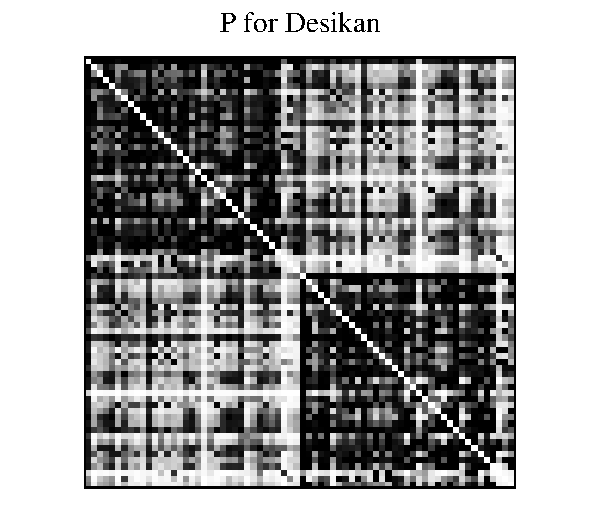
\includegraphics[height=.2\textheight]{../../figs/P_desikan.pdf} \hspace{-35pt}
%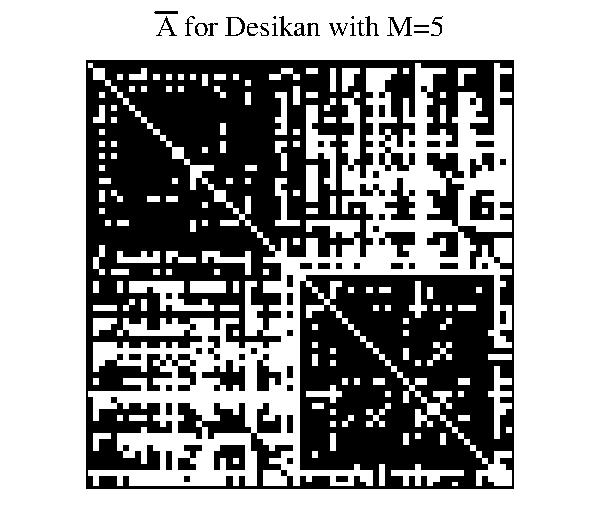
\includegraphics[height=.201\textheight]{../../figs/Abar_desikan_m1.pdf} \hspace{-35pt}
%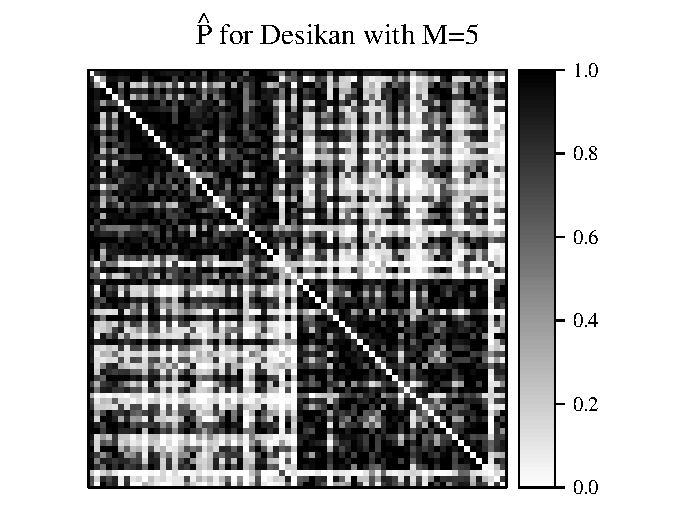
\includegraphics[height=.205\textheight]{../../figs/Phat_desikan_m1.pdf}
%\caption{{\bf Heat maps of the population mean, the sample mean, and the estimator $\hat{P}$.}
%These heat maps indicate the population mean for the $454$ graphs (left), sample mean for the 1 sampled graph (center), and $\hat{P}$ for the 1 sampled graph with dimension $d=12$ selected using the Zhu and Ghodsi method (right).
%Darker pixels indicate a higher probability of an edge between the given vertices.
%Note that $\hat{P}$ appears to better estimate the true probability matrix $P$, especially for edges between the two hemispheres, in the upper right and corresponding lower left block.
%}
%\label{fig:Matrix_desikan_m1}
%\end{cframed}
%\end{figure}
%
%\clearpage
\end{document}
